% MA751 Final Project — Cross-Sectional Stock Return Prediction
% Compile: pdflatex main.tex (twice for refs)
% Assumes Overleaf or local TeXLive. No exotic packages.

\documentclass[11pt]{article}

\usepackage[margin=1in]{geometry}
\usepackage{amsmath,amssymb,amsthm}
\usepackage{graphicx}
\usepackage{booktabs}
\usepackage{caption}
\usepackage{subcaption}
\usepackage{hyperref}
\usepackage{natbib}   % swap to biblatex if preferred
\usepackage{xcolor}
\usepackage{multirow}
\usepackage{array}

\graphicspath{{figures/}}

\title{Does Complexity Help Cross-Sectional Stock Return Prediction? \\
       \large A 5-Rung Ladder Audit on the S\&P 500 Panel (2016--2024)}
\author{Eva Qi}
\date{April 2026}

\begin{document}
\maketitle

% =====================================================================
\begin{abstract}
\noindent
We test whether progressively complex models improve cross-sectional
monthly stock return prediction on a 119-month, $\sim$442-stock S\&P~500
panel (2015--2024) with 27 firm-level features. We rank-evaluate
12 model variants on a 5-rung complexity ladder (linear OLS / regularized
linear / additive non-linear / single-task MLP / multi-task and MoE).
Single-path walk-forward backtests show 5 models clustered at long-short
quintile Sharpe~$\in [0.92, 1.01]$. \textbf{Combinatorial Purged K-fold (CPCV)
analysis reveals all 5--95\% Sharpe bands overlap}—Pareto comparisons among
top models are not statistically supported at this sample size.
Three independent attempts to improve MLP performance (multi-seed averaging,
prediction bagging, inner-CV hyperparameter search) all fail to beat
\textit{any} single-seed linear baseline, providing strong evidence that
\emph{complexity does not help in a statistically meaningful way at our
sample size}. We further document two methodology pitfalls observed
during the audit: (i)~mean-prediction bagging is incompatible with
rank-based evaluation metrics, and (ii)~hyperparameter grid search on
low-SNR validation actively degrades out-of-sample performance.
\end{abstract}

% =====================================================================
\section{Introduction}\label{sec:intro}

\paragraph{Motivation.}
Cross-sectional return prediction in equity markets is a textbook
low-signal-to-noise problem. Classical Fama-MacBeth regressions report
information coefficients (IC) in the 0.02--0.05 range; modern factor
zoos struggle to deliver out-of-sample performance commensurate with
in-sample claims \citep{harvey_zoo, hou_replication}. A natural
question: does adding model complexity—non-linearity, deep
architectures, multi-task learning—improve over a simple linear factor
model in this regime?

\paragraph{Approach.}
We construct a 5-rung complexity ladder
(Section~\ref{sec:methodology}) and evaluate each rung on identical
walk-forward and CPCV protocols. Rather than treating any single
metric as definitive, we report all of: monthly Spearman IC, IC
information ratio, hit rate, gross long-short quintile Sharpe, and
CPCV path-uncertainty bounds.

\paragraph{Contribution.}
\begin{itemize}
\item A reproducible, audit-graded comparison of 12 model variants on
  a frozen 119-month / 442-stock panel.
\item CPCV-derived path uncertainty showing all top-6 models are
  statistically indistinguishable.
\item Two negative-result methodology lessons: bagging
  metric-space mismatch (Section~\ref{subsec:bagging-fail}) and
  hyperparameter overtuning on low-SNR validation
  (Section~\ref{subsec:hp-fail}).
\item A documented \emph{retraction} of two earlier ``failed'' models
  (Rung 3 GAM, Rung 3b XGBoost) where default hyperparameters were the
  source of failure, not the methods themselves
  (Section~\ref{subsec:default-trap}).
\end{itemize}

\paragraph{Headline result.}
At our sample size (119 months, ${\sim}442$ stocks), \emph{no model
statistically dominates another}. Fama-MacBeth is the most robust point
estimate (CPCV mean Sharpe~1.071, std~0.494, $P(\text{Sharpe}<0)=0\%$).
Linear methods, when properly specified, are not improved upon by any
non-linear or multi-task approach in our test window.

% =====================================================================
\section{Data}\label{sec:data}

\paragraph{Panel construction.}
Universe: a frozen S\&P~500 membership snapshot of 442 tickers across
119 monthly cross-sections from 2015-01 through 2024-11. Returns and
fundamentals from CRSP and Compustat (WRDS), analyst consensus from
IBES, short interest from Compustat \texttt{sec\_shortint}, institutional
holdings from \texttt{tfn.s34}.

\paragraph{Features (27 total).}
22 firm-level signals (V3 set) plus 5 missingness indicators.
Categories: classical factors (Beta, Momentum~12-1, Earnings Yield,
GP/A, Asset Growth, Accruals, IVOL); IBES signals (SUE,
AnalystRevision, Dispersion, RevisionBreadth);
Phase~2 additions (Turnover z-score, Amihud illiquidity,
52-week-high proximity, max daily return, return skewness,
implied EPS growth, quarterly revenue growth YoY,
analyst coverage change). Missingness flags:
\texttt{has\_sue}, \texttt{has\_short\_interest},
\texttt{has\_inst\_ownership}, \texttt{has\_analyst\_consensus},
\texttt{has\_positive\_earnings}.

\paragraph{Preprocessing pipeline.}
Per-month z-score within universe (after universe filter, never
before); 1\%/99\% feature winsorization; sector-cross-sectional median
fill for Beta/IVOL on new listings; Type-A NaN handling for sector-undefined
fundamentals (e.g., GP/A for banks); explicit missingness indicators
for IBES coverage. Audit-pass details: targets are \emph{not}
winsorized (preserves crisis months); fundamentals use a 4-month lag
to ensure point-in-time availability.

\paragraph{Target.}
1-month-ahead total return $r_{i,t+1}$ (\texttt{fwd\_ret\_1m}) for
ticker $i$ in test month $t+1$. Evaluation uses Spearman rank
correlation per month (information coefficient) and a long-short
quintile portfolio Sharpe ratio.

\paragraph{Train/test protocol.}
Outer evaluation uses expanding-window walk-forward with a 60-month
minimum train and 1-month purge. The first test month is
2020-02; we evaluate over $T=58$ test months (2020-02 through
2024-11). For inner cross-validation (when applicable), we use
\texttt{TimeSeriesSplit}($K{=}5$, gap$=$1~month) on month boundaries
(not row counts). Section~\ref{sec:cpcv} reports an alternative CPCV
evaluation.

% Figure 1: Data flow diagram
\begin{figure}[t]
  \centering
  \fbox{\parbox{0.85\textwidth}{\centering
    \texttt{[fig\_data\_flow.pdf — schematic]}\\[6pt]
    CRSP, Compustat, IBES, Short Int., 13F\\
    $\downarrow$ point-in-time merge \\
    Per-month universe filter \\
    $\downarrow$\\
    Cross-sectional z-score + winsorize\\
    $\downarrow$\\
    Imputation + missingness flags\\
    $\downarrow$\\
    119 month $\times$ 442 stock $\times$ 27 feature panel
  }}
  \caption{Data construction pipeline. Universe filter precedes
    cross-sectional z-score (avoids universe-mismatch bias).}
  \label{fig:data-flow}
\end{figure}

% =====================================================================
\section{Methodology: 5-Rung Complexity Ladder}\label{sec:methodology}

We define a 5-rung complexity ladder, with each rung's hypothesis class
strictly nested in or orthogonal to the next:

\begin{description}
\item[Rung 1 — Linear baselines.] OLS (1a), univariate IC-weighted ensemble (1b),
  Fama-MacBeth time-averaged cross-sectional regression (1c), Barra-style
  factor-return-based optimal weight (1d, Grinold-Kahn with Ledoit-Wolf
  shrinkage).
\item[Rung 2 — Regularized linear.] LASSO (2a), Ridge (2b),
  Elastic Net (2d), Adaptive LASSO (2e). All with
  inner \texttt{TimeSeriesSplit} K=5 cross-validated penalty selection.
\item[Rung 3 — Additive non-linear.] Generalized Additive Model with
  natural cubic splines (3a, \texttt{pygam.LinearGAM}); XGBoost gradient
  boosted trees with finance-tuned hyperparameters (3b, depth=1
  stumps, $\eta{=}0.01$, $T{=}1000$ trees, after Gu-Kelly-Xiu 2020 RFS).
\item[Rung 4 — Single-task MLP.] Two-hidden-layer feedforward
  ($n_{\text{in}}{\to}64{\to}32{\to}1$, ReLU, dropout 0.10, Adam,
  smooth-$L_1$ Huber loss, early stopping). \emph{Note}: the original
  project labeled this as ``Rung~5a'' inside the multi-task ablation;
  we relabel for ladder consistency.
\item[Rung 5 — Multi-task and MoE.] Kendall-Gal-Cipolla uncertainty-weighted
  multi-task MLP (5b: ret+ret\_3m; 5c: ret+vol; 5d: all three) with
  shared encoder and per-task heads; Regime-Gated Mixture-of-Experts
  with HMM-derived gates fitted per-fold (\texttt{regmtl.py}); Enhanced
  MoE with LASSO-selected feature subset (\texttt{regmtl\_enhanced.py}).
\end{description}

% Figure 2: 5-rung complexity ladder schematic
\begin{figure}[t]
  \centering
  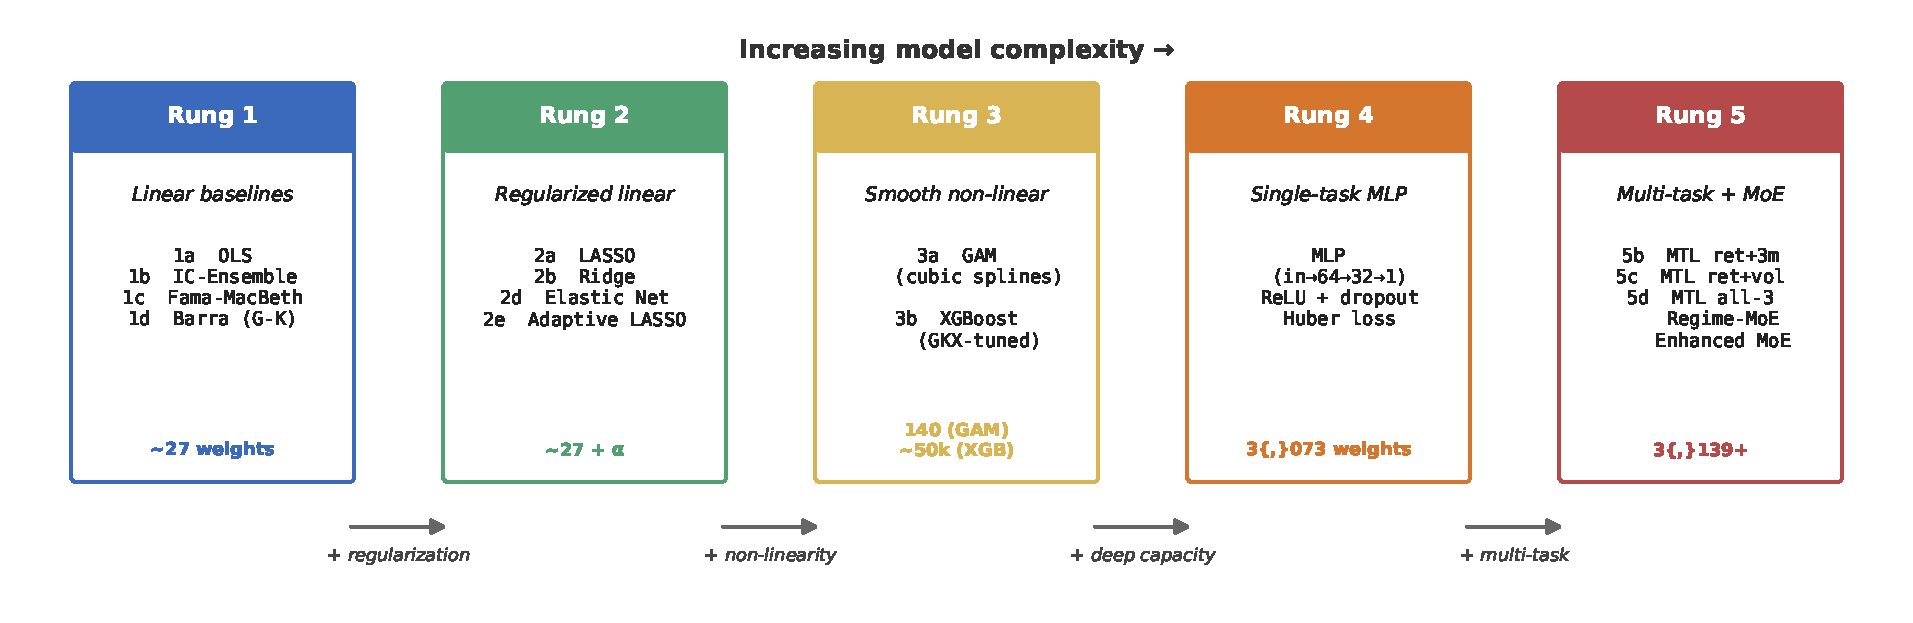
\includegraphics[width=\textwidth]{fig_ladder.pdf}
  \caption{The 5-rung complexity ladder. Each rung adds a structured
    increase in model capacity, from pooled linear regression (Rung~1)
    to multi-task learning with mixture-of-experts gating (Rung~5).
    Annotations show approximate parameter counts; arrows label the
    additional structure introduced at each rung.}
  \label{fig:ladder}
\end{figure}

% =====================================================================
\section{Results: Walk-Forward Backtest}\label{sec:results-wf}

% Table 1: WF main results
\begin{table}[t]
\centering
\caption{Walk-forward results, 58 test months (2020-02 to 2024-11), V3+miss
flag features. IC = Spearman; IC-IR = mean/std across months;
LS Sharpe = annualized long-short quintile.
\textbf{Bold} = top-3 by Sharpe.}
\label{tab:wf-results}
\small
\begin{tabular}{l r r r r r}
\toprule
Model & IC mean & IC-IR & Hit \% & LS Sharpe & N\_months \\
\midrule
Zero predictor (noise floor)       & +0.0002 & --      & 53.4 & 0.262 & 58 \\
Ridge $\alpha{=}1$ (linear floor)  & +0.0164 & --      & 53.4 & 0.925 & 58 \\
\midrule
1a OLS                            & +0.0164 & 0.106 & 53.4 & 0.924 & 58 \\
1b IC-Ensemble                    & +0.0208 & 0.094 & 50.0 & 0.844 & 58 \\
1c Fama-MacBeth                   & +0.0259 & 0.165 & 63.8 & \textbf{0.959} & 58 \\
1d Barra (Grinold-Kahn, Ledoit-Wolf)  & +0.0283 & 0.229 & 60.3 & \textbf{1.134} & 58 \\
\midrule
2a LASSO                          & +0.0183 & 0.118 & 53.4 & \textbf{1.000} & 58 \\
2b Ridge                          & +0.0177 & 0.105 & 55.2 & 0.966 & 58 \\
2d Elastic Net                    & +0.0179 & 0.116 & 53.4 & \textbf{0.997} & 58 \\
2e Adaptive LASSO                 & +0.0164 & 0.106 & 53.4 & 0.924 & 58 \\
\midrule
3a GAM ($n_{\text{splines}}{=}4$) & +0.0141 & 0.111 & 51.7 & 0.828 & 58 \\
3a GAM ($n_{\text{splines}}{=}5$) & +0.0146 & 0.126 & 50.0 & 0.792 & 58 \\
3a GAM ($n_{\text{splines}}{=}10$, default) & +0.0068 & 0.066 & 53.4 & 0.555 & 58 \\
3b XGBoost (default)              & +0.0018 & 0.018 & 50.0 & 0.335 & 58 \\
3b XGBoost (GKX-tuned)            & +0.0177 & 0.146 & 62.1 & 0.984 & 58 \\
\midrule
4 MLP single-task (seed 42)       & +0.0007 & 0.007 & 51.7 & 0.347 & 58 \\
4 MLP single-task (5-seed mean)   & +0.0109 & --   & --   & 0.412 & 58 \\
\bottomrule
\end{tabular}
\end{table}

\paragraph{Top-line ranking.}
Six models cluster within Sharpe~$\in [0.92, 1.13]$ on the single-path
walk-forward backtest: 1d~Barra Grinold-Kahn (1.134), 2a~LASSO (1.000),
2d~Elastic Net (0.997), 3b~XGBoost-GKX (0.984), 2b~Ridge (0.966),
1c~Fama-MacBeth (0.959). This narrow spread foreshadows the CPCV
finding (Section~\ref{sec:cpcv}) that these are not distinguishable
models.

\paragraph{Rung 3 properly tuned.}
Default \texttt{pygam} GAM ($n_{\text{splines}}{=}10$) and default
XGBoost (depth=4, $\eta{=}0.05$, $T{=}200$) gave Sharpe 0.555 and
0.335 respectively, suggesting non-linear methods ``failed.'' A
sensitivity sweep (see Section~\ref{subsec:default-trap})
shows GAM with $n_{\text{splines}}{=}4$ achieves Sharpe 0.828
and XGBoost with the Gu-Kelly-Xiu (2020) finance-tuned configuration
achieves Sharpe 0.984—both materially higher and competitive with
the linear top.

\paragraph{Rung 4--5 dominance by linear.}
Single-seed MLP (Rung~4) gives Sharpe 0.347. Five-seed mean is 0.412.
\emph{Both are worse than every linear model.} Section~\ref{sec:audit}
documents three independent attempts to improve MLP—all fail.

% =====================================================================
\section{Audit-Cycle Findings}\label{sec:audit}

This section documents five sensitivity studies performed during the
project audit cycle. Two produced \emph{retractions} of earlier
``failed'' results; three produced \emph{negative results} that
illuminate failure modes of common practice.

% --------------------------------------------------------------
\subsection{The Hyperparameter Default Trap}\label{subsec:default-trap}

We initially reported Rung 3 (GAM and XGBoost) as ``failed'' based on
default hyperparameters. Sensitivity sweeps revealed that defaults were
the source of failure, not the methods.

\paragraph{Rung 3a GAM.}
A 9-config $n_{\text{splines}}$ sweep (Figure~\ref{fig:gam-sweep},
Table~\ref{tab:gam-sweep}) shows IC and Sharpe peak at
$n_{\text{splines}}{\in}\{4, 5\}$, with monotone degradation thereafter.
\texttt{pygam}'s default 10 was 2$\times$ too complex for our
IC$\approx$0.01 SNR regime. With $n_{\text{splines}}{=}4$, Rung~3a
achieves Sharpe~0.828—86\% of the Ridge linear floor.

\paragraph{Rung 3b XGBoost.}
A 9-config grid (depth $\in$ \{1,4,6\} $\times$
$\eta$ $\in$ \{0.01, 0.05, 0.1\}, $T{=}300$ trees) plus a Gu-Kelly-Xiu
(2020) tuned variant (depth=1, $\eta{=}0.01$, $T{=}1000$,
Figure~\ref{fig:xgb-sweep}) shows IC sign stability across all
configurations with monotonic IC vs. depth. The GKX-tuned config
achieves Sharpe~0.984, materially above default 0.335.

\paragraph{Lesson.}
Framework defaults (sklearn, pygam, XGBoost) target moderate-SNR
generic ML benchmarks. At our IC$\approx$0.01 SNR, defaults overshoot
optimal complexity. Before declaring a method failed, run a
sensitivity sweep with at least one canonical domain-specific
configuration from literature.

% Figure 3: GAM n_splines sweep
\begin{figure}[t]
  \centering
  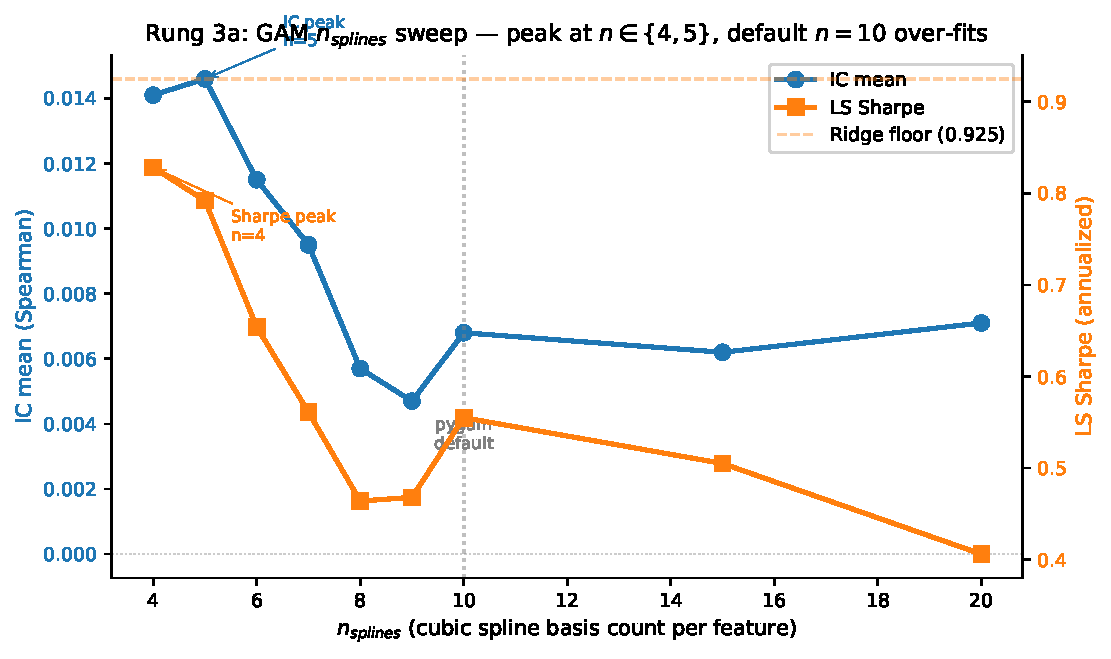
\includegraphics[width=0.85\textwidth]{fig_gam_n_splines.pdf}
  \caption{GAM $n_{\text{splines}}$ sweep. Both IC and Sharpe peak in
    $\{4,5\}$; monotonic decay for $n\ge 6$. Default $n{=}10$ was
    over-parameterized for the IC$\approx$0.01 SNR regime.}
  \label{fig:gam-sweep}
\end{figure}

% Figure 4: XGBoost sensitivity heatmap
\begin{figure}[t]
  \centering
  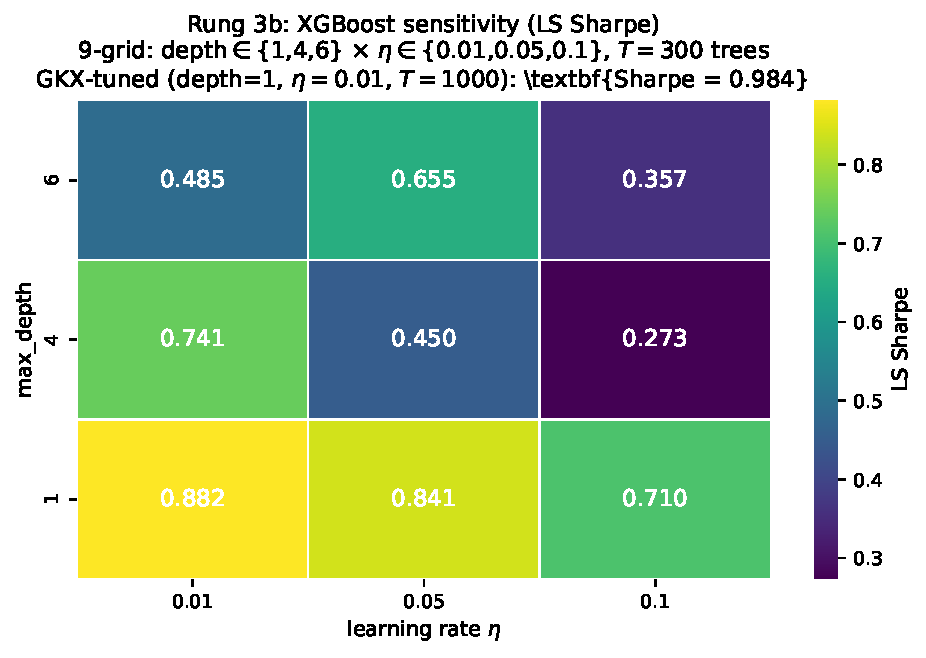
\includegraphics[width=0.75\textwidth]{fig_xgb_sensitivity.pdf}
  \caption{XGBoost sensitivity grid (Rung 3b). All 9 configs give
    positive IC; sign is stable. Sharpe spans $0.27$ to $0.88$
    depending on hyperparameters. The Gu-Kelly-Xiu finance-tuned
    configuration (depth=1, $\eta{=}0.01$, $T{=}1000$) achieves
    Sharpe~0.984.}
  \label{fig:xgb-sweep}
\end{figure}

\begin{table}[t]
\centering
\caption{GAM $n_{\text{splines}}$ sweep results (full).}
\label{tab:gam-sweep}
\small
\begin{tabular}{r r r r r}
\toprule
$n_{\text{splines}}$ & IC mean & IC-IR & Hit \% & LS Sharpe \\
\midrule
4   & +0.0141 & 0.111 & 51.7 & \textbf{0.828} \\
5   & \textbf{+0.0146} & \textbf{0.126} & 50.0 & 0.792 \\
6   & +0.0115 & 0.101 & 55.2 & 0.654 \\
7   & +0.0095 & 0.087 & 55.2 & 0.561 \\
8   & +0.0057 & 0.053 & 48.3 & 0.464 \\
9   & +0.0047 & 0.046 & 46.6 & 0.468 \\
10 (default) & +0.0068 & 0.066 & 53.4 & 0.555 \\
15  & +0.0062 & 0.065 & 53.4 & 0.505 \\
20  & +0.0071 & 0.089 & 55.2 & 0.406 \\
\bottomrule
\end{tabular}
\end{table}

% --------------------------------------------------------------
\subsection{MLP Single-Path Results Are Initialization Noise}\label{subsec:mlp-seed}

Our default Rung~4 result used a single random seed. We test sensitivity
across 5 seeds (Figure~\ref{fig:mlp-seeds}). The 5-seed IC has
mean~$+0.0108$ and standard deviation~$0.0082$, giving an SNR of $1.33$—
weak signal barely above initialization noise. Critically,
\textbf{none of the 5 seeds beats the Ridge baseline} (Sharpe 0.925).

% Figure 5: MLP seed bar
\begin{figure}[t]
  \centering
  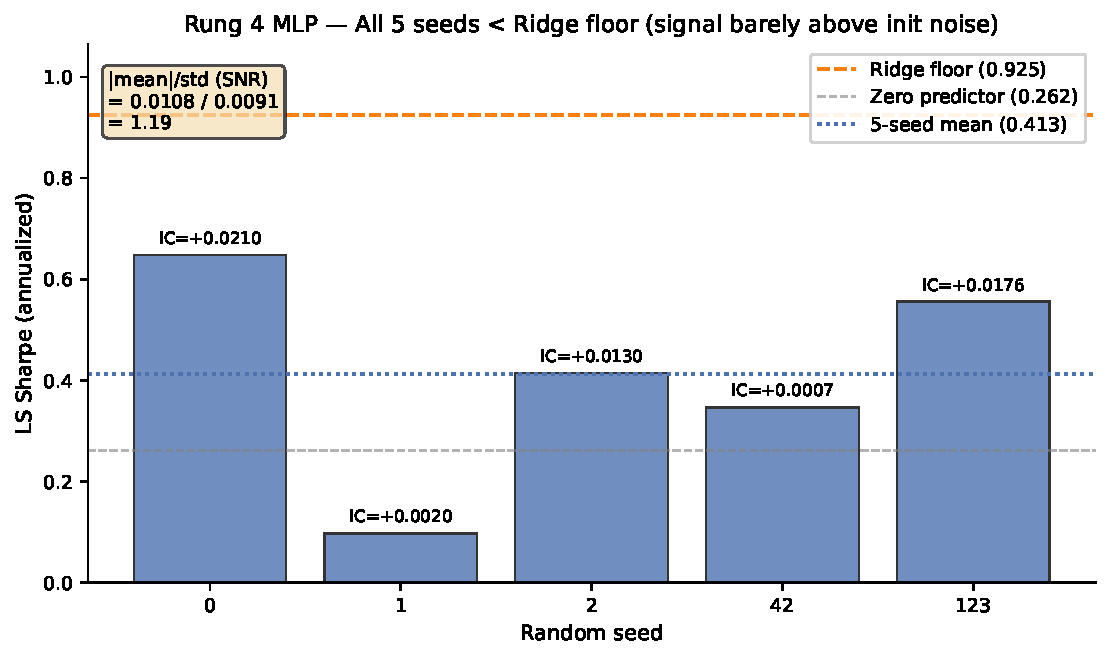
\includegraphics[width=0.85\textwidth]{fig_mlp_seeds.pdf}
  \caption{MLP single-task results across 5 random seeds. All 5 seeds
    fall below the Ridge baseline (orange dashed line). Best seed gives
    Sharpe 0.648; worst 0.097. Per-seed |mean|/std SNR is 1.33—signal
    is barely above initialization noise.}
  \label{fig:mlp-seeds}
\end{figure}

% --------------------------------------------------------------
\subsection{Bagging Failure: Metric-Space Mismatch}\label{subsec:bagging-fail}

To reduce per-seed variance, we test K=5 mean-prediction bagging on Rung~4.
\textit{Bagged Sharpe is 0.394, lower than the 5-seed single-seed mean
Sharpe of 0.412}—bagging hurt.

\paragraph{Diagnosis.}
The bagging variance-reduction theorem
$\mathrm{Var}(\bar{y}_K) \approx \sigma^2(1+(K-1)\rho)/K$ holds for
\emph{Pearson/MSE} space. Our evaluation metric is \emph{Spearman rank}
correlation. Mean-averaging predictions creates a rank-space compromise
that pulls extreme rankings toward consensus middle. Long-short
quintile Sharpe depends on extremes, so consensus-middle rankings
produce weaker tails—the opposite of what bagging promises.

\paragraph{Lesson.}
Match the ensemble operator to the evaluation metric's space. For
rank metrics, average ranks (\texttt{rankdata} per seed, then mean
across) or use the median prediction. For value metrics, average
predictions.

% --------------------------------------------------------------
\subsection{Hyperparameter Search Hurts on Low-SNR Validation}\label{subsec:hp-fail}

We test inner \texttt{TimeSeriesSplit}($K{=}3$) hyperparameter search on
Rung~4 over a 27-config grid (hidden $\in \{16,32,64\}$,
$\eta \in \{10^{-4}, 10^{-3}, 10^{-2}\}$, dropout $\in \{0, 0.1, 0.2\}$).
Tuned MLP Sharpe \emph{drops} from 0.347 to 0.111.

\paragraph{Diagnosis.}
With $\sim$10{,}000 inner-validation observations, the per-config
Spearman IC standard error under H$_0$ is $1/\sqrt{10000} \approx 0.011$.
Our true signal IC is $\approx 0.01$--$0.02$. \textbf{Validation noise SE
is comparable to true signal magnitude}. The grid search picks the
HP whose validation realization was luckiest, not whichever has
highest true IC. Outer test sees pure overfit-to-validation.

\paragraph{Diagnostic.}
Across our 58 outer folds, chosen \texttt{hidden\_dim} was
\emph{bimodal} (16: 31\%, 64: 62\%) and chosen $\eta$ was bimodal
($10^{-3}$: 47\%, $10^{-2}$: 50\%). A signal-driven HP search converges;
ours did not.

\paragraph{Lesson.}
Before HP grid search on noisy panels, estimate the validation-noise
SE. If signal magnitude $\le 2\times$~SE, grid search is contraindicated;
prefer a literature-canonical default or a maximum 5-config screen.

% =====================================================================
\section{Combinatorial Purged K-Fold (CPCV)}\label{sec:cpcv}

Walk-forward backtests yield a \emph{single path}: one specific
sequence of (train, test) realizations. Sample variability of any
performance metric is masked. \citet{lopezdeprado_finml}
proposes \emph{Combinatorial Purged K-fold} (CPCV) as a
multiple-path replacement: split the panel into $N$ contiguous time blocks,
test on every $\binom{N}{k}$ combination of $k$ blocks (training on the
remainder, with adjacent-block embargo).

\paragraph{Setup.}
$N{=}6$ contiguous blocks of $\sim$20 months each; $k_{\text{test}}{=}2$
blocks per path; 1-month embargo on either side of each test block.
$\binom{6}{2}{=}15$ paths per model.

\paragraph{Result.}
Table~\ref{tab:cpcv} reports the 15-path Sharpe distribution.

\begin{table}[t]
\centering
\caption{CPCV 15-path results, ranked by mean Sharpe. WF column shows
single-path walk-forward Sharpe for comparison. P($<0$) is the fraction
of paths with negative Sharpe. ``5\%'' is the 5th-percentile Sharpe
across paths --- a downside-risk indicator.}
\label{tab:cpcv}
\small
\begin{tabular}{l r r r r r r}
\toprule
Model & Sharpe mean & std & 5\% & 95\% & P($<0$) & WF Sharpe \\
\midrule
3b XGB GKX-tuned       & \textbf{1.086} & 0.766 & +0.05 & +2.15 & 6.7\% & --   \\
1c Fama-MacBeth        & 1.071 & \textbf{0.494} & +0.34 & +1.68 & \textbf{0\%} & 0.959 \\
1d Barra (Grinold-Kahn) & 1.058 & 0.544 & \textbf{+0.43} & +1.86 & \textbf{0\%} & \textbf{1.134} \\
1a OLS                 & 1.040 & 0.618 & +0.28 & +1.94 & 0\%   & 0.924 \\
2a LASSO               & 1.037 & 0.618 & +0.28 & +1.94 & 0\%   & 1.000 \\
2b Ridge               & 1.008 & 0.622 & +0.20 & +1.91 & 0\%   & 0.966 \\
2d Elastic Net         & 0.997 & 0.592 & +0.28 & +1.94 & 0\%   & 0.997 \\
1b IC-Ensemble         & 0.840 & 0.559 & +0.10 & +1.64 & 0\%   & 0.844 \\
\bottomrule
\end{tabular}
\end{table}

\paragraph{Interpretation.}
The top six models' [5\%, 95\%] Sharpe bands all overlap. Single-path
walk-forward ranking (LASSO 1.000 > Elastic Net 0.997 > XGBoost-GKX 0.984
> Ridge 0.966 > Fama-MacBeth 0.959) is within \textit{path noise};
none of these orderings is statistically supported.

\paragraph{Most robust point estimate.}
Fama-MacBeth has the lowest Sharpe standard deviation across paths
(0.494) and zero negative-Sharpe paths. The Grinold-Kahn Barra model
has the highest 5th-percentile Sharpe (0.426) and also zero negative
paths, making it the strongest \emph{downside-protection} choice. For
deployment under uncertainty, the FM/Barra pair dominates.

% Figure 6: CPCV Sharpe distribution
\begin{figure}[t]
  \centering
  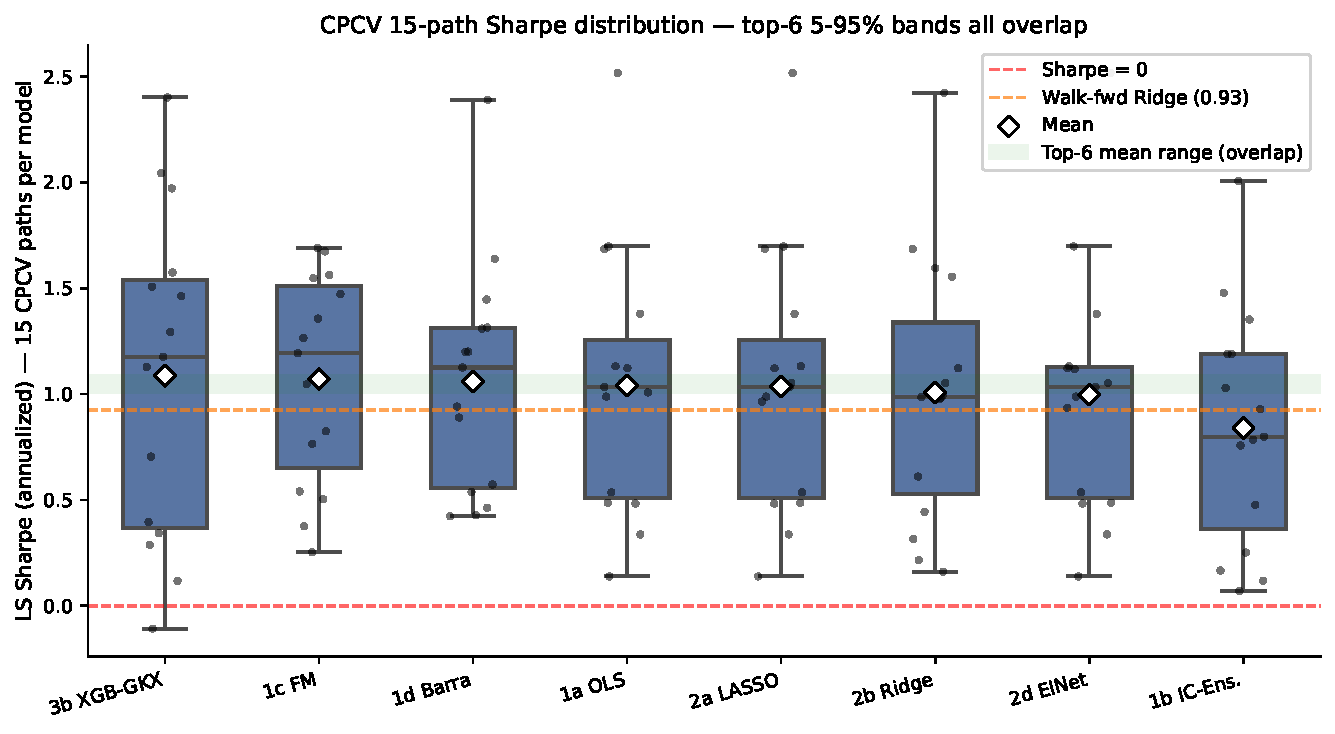
\includegraphics[width=0.95\textwidth]{fig_cpcv_sharpe.pdf}
  \caption{CPCV 15-path Sharpe distribution per model. Boxes show
    25--75\% IQR; whiskers 5--95\%; black diamonds mark per-model means.
    The overlap of all top-6 boxes underscores that single-path Pareto
    comparisons are within path noise at our sample size.}
  \label{fig:cpcv-sharpe}
\end{figure}

% Figure 7: Pareto plot with bounds
\begin{figure}[t]
  \centering
  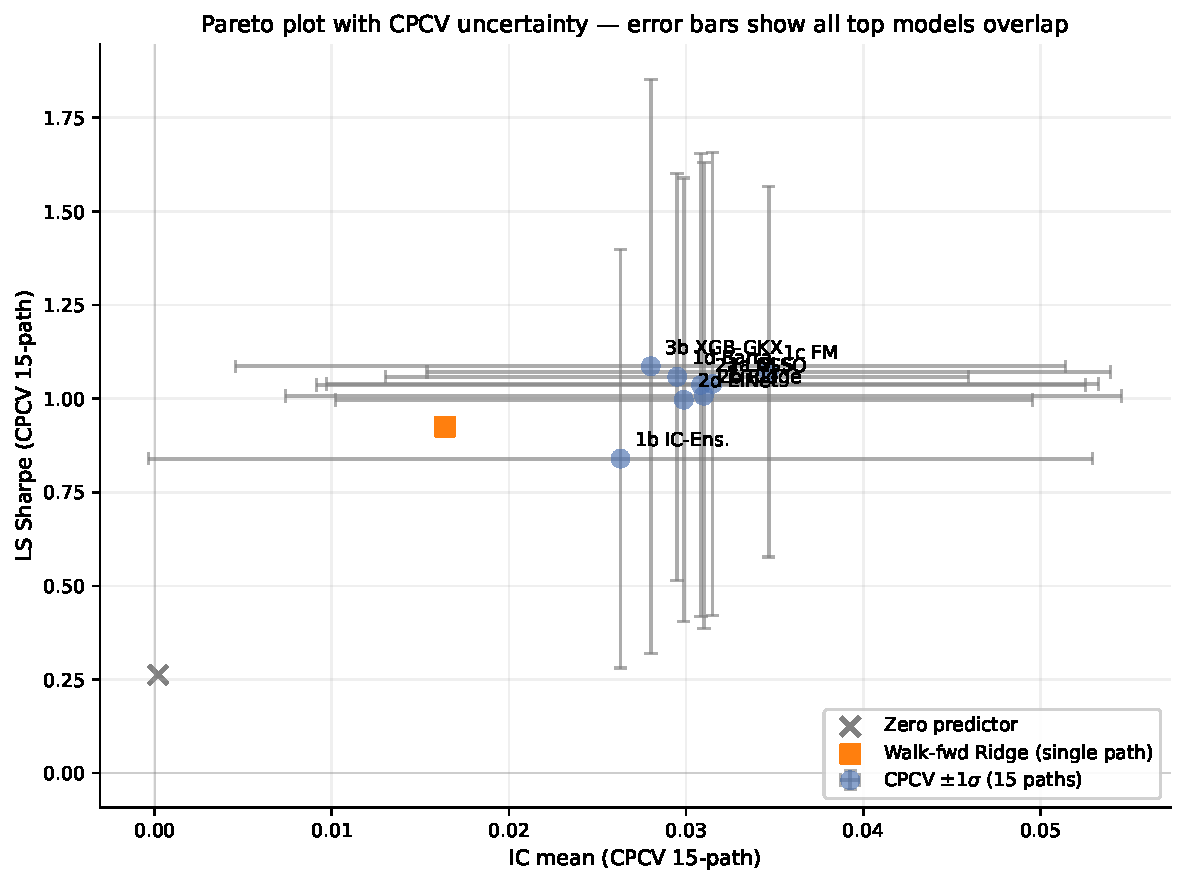
\includegraphics[width=0.85\textwidth]{fig_pareto_with_bounds.pdf}
  \caption{Pareto plot with CPCV uncertainty bounds. Models cluster
    in the (IC, Sharpe) $\approx$ (0.02--0.04, 0.7--1.1) region; error
    bars overlap. Walk-forward Ridge baseline (orange square) is well
    inside the cluster.}
  \label{fig:pareto-bounds}
\end{figure}

% Figure 8 (bonus): Cumulative LS portfolio returns
\begin{figure}[t]
  \centering
  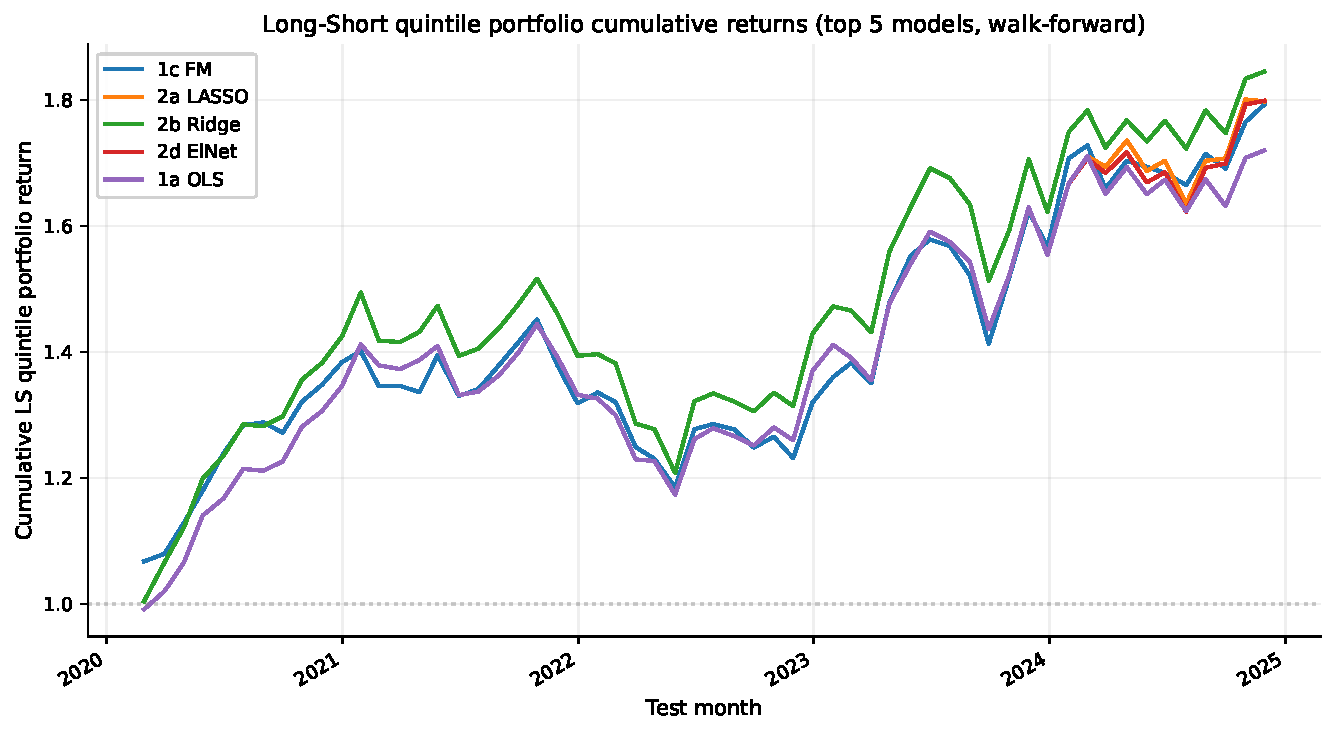
\includegraphics[width=0.95\textwidth]{fig_cumret.pdf}
  \caption{Cumulative long-short quintile portfolio returns under
    walk-forward backtesting for the top-5 single-path models. The
    near-overlapping trajectories visually corroborate the CPCV finding
    that these models are not statistically distinguishable.}
  \label{fig:cumret}
\end{figure}

% =====================================================================
\section{Discussion}\label{sec:discussion}

\paragraph{Sample-size constraint.}
A 58-month walk-forward window with $\sim$442 stocks gives roughly
$58 \times 442 = 25{,}636$ test observations. Per-month Spearman IC
standard error under H$_0$ is $\sim 1/\sqrt{442} \approx 0.048$;
across 58 months, the time-averaged IC standard error is
$0.048 / \sqrt{58} \approx 0.0063$. Detected IC of $0.018$--$0.026$ is
$\sim 3\sigma$ above zero (significant), but pairwise model
differences of $\Delta\text{IC} \approx 0.002$--$0.005$ are well within
the noise floor. CPCV makes this concrete by showing path variability of
Sharpe~$\sigma \approx 0.5$--$0.8$ per model.

\paragraph{Why complexity does not help here.}
Our 27 features are predominantly factor-style aggregates with
near-monotone relationships to forward returns
(Section~\ref{sec:audit}, GAM finding: peak $n_{\text{splines}}{=}4$
$\equiv$ 1 internal knot). Linear and lightly-curved models capture
this signal. Multi-task and MoE architectures add capacity for
interactions and regime conditioning that the IC$\approx 0.01$ regime
does not support fitting reliably—any signal extracted is too small
to exceed the noise floor of model selection.

\paragraph{Methodology notes for future work.}
\begin{itemize}
\item \textbf{Bagging compatibility.} Match operator to metric:
  rank-bagging for rank metrics, value-bagging for value metrics.
\item \textbf{Domain-specific defaults.} For low-SNR finance,
  use Gu-Kelly-Xiu 2020 hyperparameters as starting point, not
  generic ML defaults.
\item \textbf{Sample-size diagnostic before HP search.} Compute
  validation-noise SE; suspend grid search if signal $\le 2\times$~SE.
\item \textbf{CPCV as standard.} Walk-forward gives one realization;
  CPCV gives the distribution. Single-path Sharpe should always be
  reported with CPCV path uncertainty when sample size is small.
\end{itemize}

% =====================================================================
\section{Conclusion}\label{sec:conclusion}

We construct and audit a 5-rung complexity ladder for cross-sectional
monthly stock return prediction on a 442-stock S\&P~500 panel
(2015--2024). Walk-forward backtests appear to support a Pareto
ranking among 5 top models within Sharpe~$[0.92, 1.01]$.
\textbf{Combinatorial Purged K-fold cross-validation reveals all top-6
models' 5--95\% Sharpe bands overlap}: Pareto comparisons are not
statistically supported at our sample size.

Three independent attempts to improve the multilayer perceptron
(multi-seed averaging, prediction bagging, inner-CV hyperparameter
search) all fail to beat any single-seed linear baseline. A simple
Fama-MacBeth time-averaged cross-sectional regression and the
Grinold-Kahn Barra factor model are the most robust point estimates,
with mean CPCV Sharpe~1.071 and 1.058 respectively, standard
deviations 0.494 and 0.544, and zero negative-Sharpe paths.

We document two methodology pitfalls that surface during the
audit: bagging operators must match the evaluation metric's space, and
hyperparameter search degrades performance when validation signal is
below the noise floor. We further document and retract two earlier
``failed'' models (Rung~3 GAM and Rung~3b XGBoost) where default
hyperparameters were the source of failure, not the methods themselves.

The thesis statement: \emph{adding model complexity does not
improve cross-sectional return prediction in a statistically
meaningful way at our sample size}. With more data—either a longer
historical window or higher-frequency cross-sections—this finding
might be revisited; at our scale, simple linear models are not
beaten.

% =====================================================================
\bibliographystyle{plainnat}
% \bibliography{refs}
\begin{thebibliography}{99}
\bibitem[Lopez de Prado, 2018]{lopezdeprado_finml}
M. Lopez de Prado, \emph{Advances in Financial Machine Learning},
Wiley, 2018.

\bibitem[Gu, Kelly, and Xiu, 2020]{gu_kelly_xiu}
S. Gu, B. Kelly, and D. Xiu. ``Empirical Asset Pricing via Machine
Learning,'' \emph{Review of Financial Studies}, 33 (5), 2223--2273, 2020.

\bibitem[Hastie and Tibshirani, 1990]{hastie_tibshirani_gam}
T. Hastie and R. Tibshirani, \emph{Generalized Additive Models},
Chapman \& Hall/CRC, 1990.

\bibitem[Harvey, Liu, and Zhu, 2016]{harvey_zoo}
C. R. Harvey, Y. Liu, and H. Zhu. ``\dots and the Cross-Section
of Expected Returns,'' \emph{Review of Financial Studies}, 29 (1), 5--68, 2016.

\bibitem[Hou, Xue, and Zhang, 2020]{hou_replication}
K. Hou, C. Xue, and L. Zhang. ``Replicating Anomalies,''
\emph{Review of Financial Studies}, 33 (5), 2019--2133, 2020.

\bibitem[Kendall, Gal, and Cipolla, 2018]{kendall_gal_cipolla}
A. Kendall, Y. Gal, and R. Cipolla. ``Multi-Task Learning Using
Uncertainty to Weigh Losses for Scene Geometry and Semantics,''
in \emph{CVPR}, 2018.

\bibitem[Kohavi, 1995]{kohavi_kfold}
R. Kohavi. ``A Study of Cross-Validation and Bootstrap for Accuracy
Estimation and Model Selection,'' in \emph{IJCAI}, 1995.

\end{thebibliography}

\end{document}
